%xelatex -shell-escape -output-directory=bin ergasia.tex
\documentclass{assignment}

\usepackage{enumerate} % Για την χρησιμοποίηση roman enumerate
\usepackage{paralist} % για το περιβάλλον inparaenum που είναι οι λίστες μέσα στο κείμενο.

\title{Δίκτυα Υπολογιστών \\ 1ο Εργαστήριο: Στατική Δρομολόγηση \\ Εργασία: assign2}
\date{Αθήνα, 2015}

\author{Αναγνωστόπουλος Βασίλης - Θάνος (ΜΠΠΛ 13002) \and Βελισσαρίου Κυριάκος (ΜΠΠΛ 13005)}

\begin{document}

\maketitle
% Να σκεφτώ τί αλλαγές θέλω να κάνω με τις αριθμήσεις και άμα θέλω να κάνω.
% Να σκεφτώ να τις ενσωματώσω και στο assignment.cls

\setcounter{page}{1} 
\pagenumbering{roman}

\pagestyle{plain}
\tableofcontents
\listoftables
\listoffigures
%\renewcommand\listoflistingscaption{Κατάλογος πηγαίου κώδικα}
%\listoflistings
\newpage

%\pagestyle{headings}
%\pagestyle{fancy}
\setcounter{page}{1} 
\pagenumbering{arabic}


Δίνεται η παρακάτω τοπολογία:

\begin{center}
\resizebox*{\textwidth}{!}{
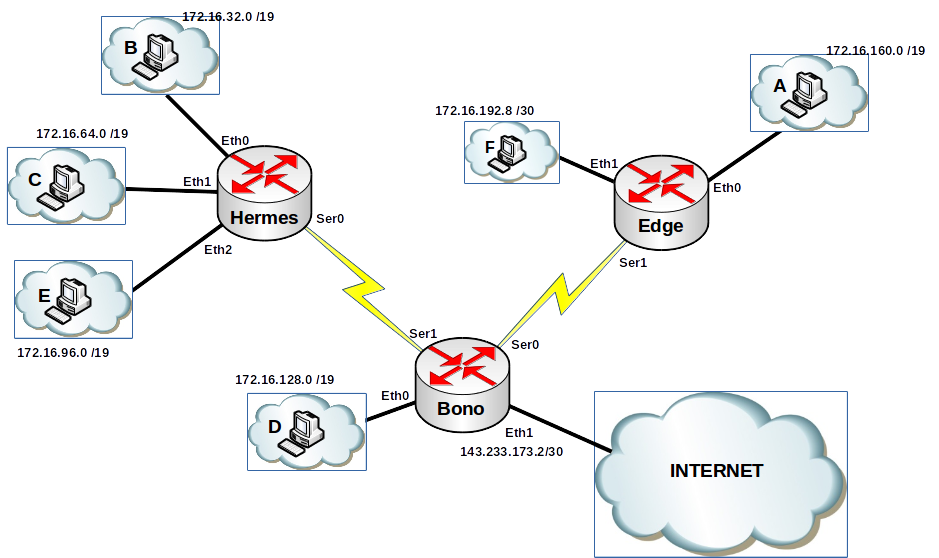
\includegraphics{images/lan.png}}
\end{center}
 
Παραδοτέα:

\begin{enumerate}
  \item Η έκθεση σας:
  \begin{enumerate}
     \item Screenshot της τοπολογίας.
     \item Screenshot που θα εμφανίζει τις επιτυχημένες προσπάθειες πρόσβασης 2 σταθμών στην υπηρεσία HTTP.
     \item Screenshot που θα αποδεικνύει το ζητούμενο 3, όπως διατυπώνεται παραπάνω.
     \item Screenshot με το αποτέλεσμα εκτέλεσης της εντολής \#show ip ospf
     \item Screenshot με το αποτέλεσμα εκτέλεσης της εντολής \#show ip ospf database
  \end{enumerate}
  \item Τα αρχεία (.pkt) με την τοπολογία σας.
\end{enumerate}

Ζητούμενα:


\section{Άσκηση 1η}
\subsection{Εκφώνηση}

Screenshot της τοπολογίας.

\subsection{Λύση}
\begin{center}
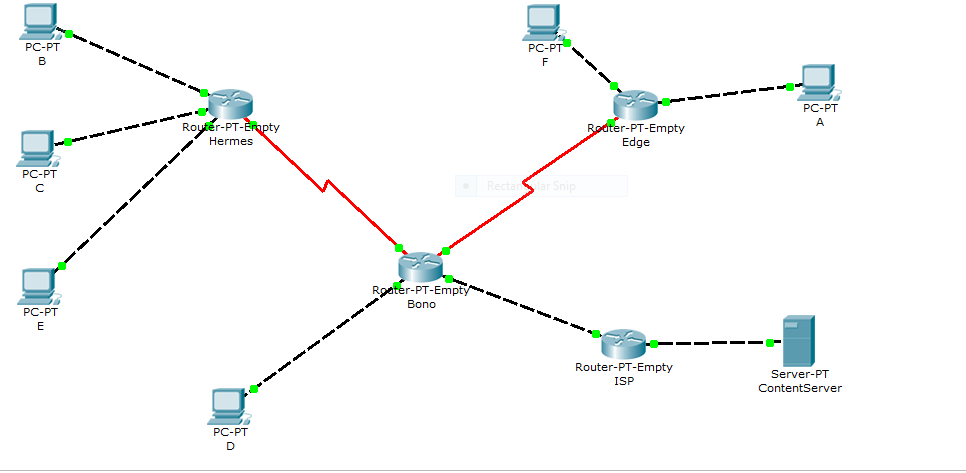
\includegraphics[width=\textwidth, height=\textheight, keepaspectratio]{images/topology.png}
\end{center}

\section{Άσκηση 2η}
\subsection{Εκφώνηση}
Screenshot που θα εμφανίζει τις επιτυχημένες προσπάθειες πρόσβασης 2 σταθμών στην υπηρεσία HTTP.

\subsection{Λύση}
Για να είναι δυνατή η πρόσβαση των σταθμών στον στην υπηρεσία http και μόνο σε
αυτή, εφαρμόστηκε στο interface Fa8/0 του Bono η εξής ACL:
\captionof{listing}{ACL για το β'}
\begin{minted}[breaklines=true, frame=lines, framesep=2mm, baselinestretch=1.2, fontsize=\footnotesize, linenos]{bash}
permit tcp any any eq www
\end{minted}

Ακολουθούν screenshot από επιτυχημένες προσπάθειες δύο σταθμών στην υπηρεσία
http.
\begin{center}
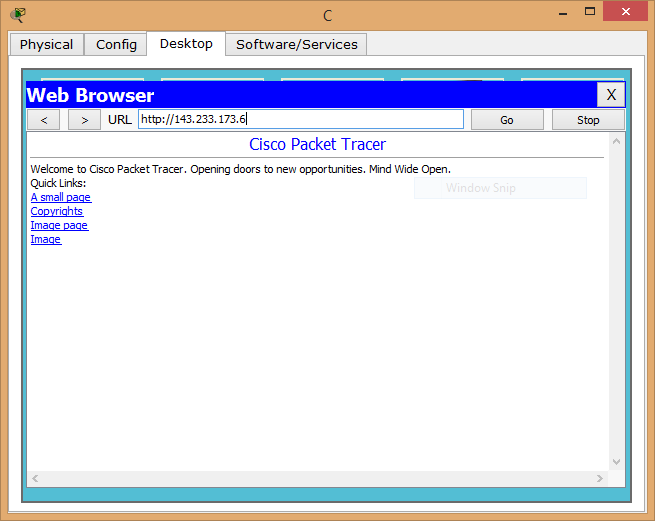
\includegraphics[width=\textwidth, height=\textheight, keepaspectratio]{images/http1.png}
\end{center}

\begin{center}
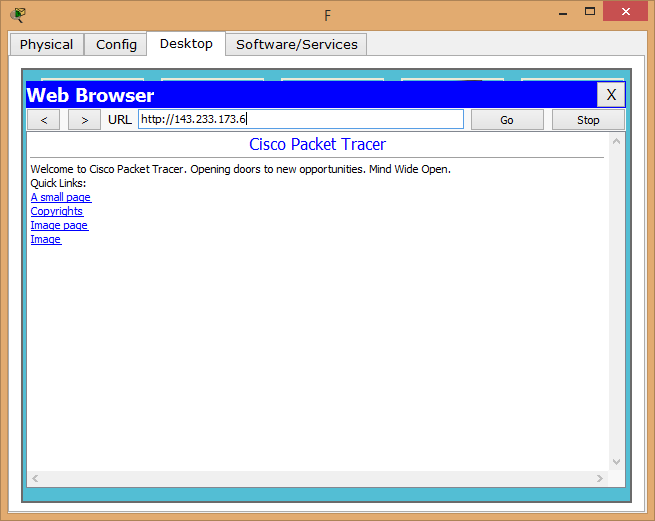
\includegraphics[width=\textwidth, height=\textheight, keepaspectratio]{images/http2.png}
\end{center}

\section{Άσκηση 3η}
\subsection{Εκφώνηση}

Τα δίκτυα που βρίσκονται στον δρομολογητή Hermes είναι προσβάσιμα σε όλους τους άλλους μόνο σε περίπτωση χρήσης των εργαλείων ping και traceroute.

\subsection{Λύση}

\section{Άσκηση 4η}
\subsection{Εκφώνηση}

Οι δρομολογητές αξιοποιούν τον αλγόριθμο OSPF για τη διαδικασία της δρομολόγησης. 
Προς το Διαδίκτυο χρησιμοποιείται στατική δρομολόγηση.

\subsection{Λύση}

\captionof{listing}{Οι εντολές για το OSPF στον Hermes}
\begin{minted}[breaklines=true, frame=lines, framesep=2mm, baselinestretch=1.2, fontsize=\footnotesize, linenos]{bash}
Hermes(config)# router ospf 500
Hermes(config-router)# network 172.16.32.0 0.0.31.255 area 0
Hermes(config-router)# network 172.16.64.0 0.0.31.255 area 0
Hermes(config-router)# network 172.16.96.0 0.0.31.255 area 0
Hermes(config-router)# network 172.16.192.0 0.0.0.3 area 0
Hermes(config-router)# ^Z
Hermes(config)# ip route 143.233.173.0 255.255.255.252 172.16.192.1
\end{minted}

\captionof{listing}{Οι εντολές για το OSPF στον Edge}
\begin{minted}[breaklines=true, frame=lines, framesep=2mm, baselinestretch=1.2, fontsize=\footnotesize, linenos]{bash}
Edge(config)# router ospf 500
Edge(config-router)# network 172.16.192.8 0.0.0.3 area 0
Edge(config-router)# network 172.16.160.0 0.0.31.255 area 0
Edge(config-router)# network 172.16.192.4 0.0.0.3 area 0
Edge(config-router)# ^Z
Edge(config)# ip route 143.233.173.0 255.255.255.252 172.16.192.6
\end{minted}

\captionof{listing}{Οι εντολές για το OSPF στον Bono}
\begin{minted}[breaklines=true, frame=lines, framesep=2mm, baselinestretch=1.2, fontsize=\footnotesize, linenos]{bash}
Bono(config)# router ospf 500
Bono(config-router)# network 172.16.128.0 0.0.31.255 area 0
Bono(config-router)# network 172.16.192.0 0.0.0.3 area 0
Bono(config-router)# network 172.16.192.4 0.0.0.3 area 0
\end{minted}

\phantomsection \label{Βιβλιογραφία}
\addcontentsline{toc}{section}{Βιβλιογραφία}
%\mtcaddchapter[Βιβλιογραφία] % Λόγω του minitoc
\bibliographystyle{plain}
\bibliography{references}

\newpage

\end{document}

